\documentclass{beamer}
%\documentclass[handout,t]{beamer}

\batchmode
% \usepackage{pgfpages}
% \pgfpagesuselayout{4 on 1}[letterpaper,landscape,border shrink=5mm]

\usepackage{amsmath,amssymb,enumerate,epsfig,bbm,calc,color,ifthen,capt-of,float}
\usepackage{algorithm2e}
\usepackage{algorithmic}
\usepackage{movie15}
\usepackage{animate}
\usepackage{xmpmulti}
\usepackage{movie15}
\usepackage{graphicx}
\usepackage{grffile}




\usetheme{Berlin}

\usecolortheme{mit}

\title{Hierarchical Leader Election Algorithm With Remoteness Constraint}
\author{Mohamed Tbarka}
\date{\today}
\pgfdeclareimage[height=0.5cm]{mit-logo}{ensias-logo.pdf}
\logo{\pgfuseimage{mit-logo}\hspace*{0.3cm}}

\AtBeginSection[]
{
	\begingroup
	\tiny
  \begin{frame}<beamer>
    \frametitle{Outline}
    \tableofcontents[currentsection]
  \end{frame}
\endgroup
}
\beamerdefaultoverlayspecification{<+->}
% -----------------------------------------------------------------------------
\begin{document}
% -----------------------------------------------------------------------------
\setbeamerfont{Outline}{size=\tiny}

\frame{\titlepage}

\section[Outline]{}
\begingroup
\tiny
\begin{frame}{Outline}

  \tableofcontents
\end{frame}
\endgroup
% -----------------------------------------------------------------------------
\section{Introduction}
\subsection{Leader Election Problem}
\begin{frame}{What is the problem of leader election ?}
Leader election is an important primitive for distributed computing, useful as a sub-routine for any application that requires the selection of a unique processor among multiple candidate processors (video conferencing, multi-player games, ...).
\end{frame}

\begin{frame}{What is distributed computing ?}
Distributed computing is a model in which components of a software system are shared among multiple computers to improve efficiency and performance.
\end{frame}

\subsection{State of art}
\begin{frame}{State of art}
	
\begin{figure}
	\centering
	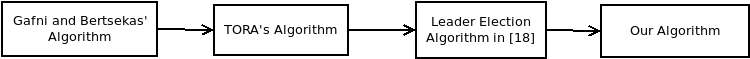
\includegraphics[width=1\linewidth]{state_of_art}
	\caption[State Of Art]{State Of Art}
	\label{fig:stateofart}
\end{figure}

\end{frame}
\iffalse
\begin{frame}{The Bully Algorithm}
  As a first example, consider the bully algorithm devised by Garcia-Molina (1982). When any process notices that the coordinator is no longer responding to requests, it initiates an election. A process, P, holds an election as follows:
  \pause
  \begin{itemize}
    \item <2-> $P$ sends an $ELECTION$ message to all processes with higher numbers.
    \item <3-> If no one responds, $P$ wins the election and becomes coordinator.
    \item <4-> If one of the higher-ups answers, it takes over. $P$'s job is done.
  \end{itemize}
\end{frame}

\begin{frame}
	\begin{figure}
		\centering
		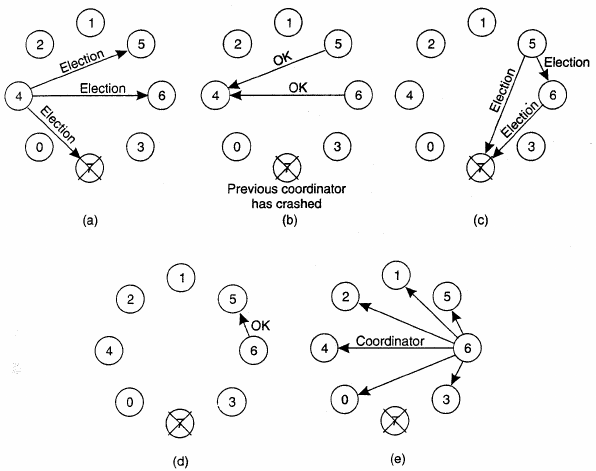
\includegraphics[width=0.7\linewidth]{bully_algorithm}
		\caption{Bully Algorithm}
		\label{fig:bullyalgorithm}
	\end{figure}
\end{frame}
\fi
% -----------------------------------------------------------------------------
\section{Preliminaries}
\subsection{System Model}

\begin{frame}{System Model}

\begin{itemize}
	\item The system is consisting of a set $P$ of computing nodes and a set $\chi$ of directed communication channels from one node to another node.
	\item The whole system as a set of (infinite) state machines that interact through shared events.

\end{itemize}

\end{frame}


\begin{frame}{Asynchronous Dynamic Links' Model}

	The state of $Channel(u, v)$, which models the communication channel from node u to node v, consists of:
	\begin{itemize}
		\item a $status_{uv}$ variable;
		\item and a queue $mqueue_{uv}$ of messages.
	\end{itemize}
	 

\end{frame}

\begin{frame}{Configurations \& Executions}

\begin{itemize}
	\item The notion of configuration is used to capture an instantaneous snapshot of the state of the entire system.
	\item A configuration is a vector of node states, one for each node in $P$, and a vector of channel states, one for each channel in $\chi$.
\end{itemize}

\end{frame}

\begin{frame}{Configurations \& Executions}
In an initial configuration:
\begin{itemize}
	\item each node is in an initial state (according to its algorithm), \item for each channel $Channel(u, v)$, $mqueue_{uv}$ is empty, and \item for all nodes $u$ and $v$, $status_{uv} = status_{vu}$ (i.e., either both channels between $u$ and $v$ are up, or both are down).
\end{itemize}
\end{frame}

\begin{frame}{Configurations \& Executions}
	An execution is an infinite sequence $C_0, e_1 ,C_1, e_2, C_2 , ...$ of alternating configurations and events, starting with an initial configuration and, if finite, ending with a configuration.
\end{frame}


\subsection{Problem Definition}
\begin{frame}{Problem Definition}
Each node $u$ in the system should have after the last topology change :
\begin{itemize}
	\item a local variable $lid_{u}$ to hold the $id$ of the supreme leader;
	\item another local variable $slid_u$ to hold the identifier of the sub-leader whose remoteness towards $u$ obeys the constraint.
\end{itemize}
\end{frame}

% -----------------------------------------------------------------------------
\section{H. Leader Election Algorithm}
\subsection{Informal Description}
\begin{frame}{Informal description}
After a leader is gone, the algorithm consists on three waves:
\pause
\begin{itemize}
	\item First wave : initiated by one of the lost leader's neighbors looking for it;
	\item Second wave : initiated by the node located at the edge of the network if the search has hit a dead-end;
	\item Third wave : initiated by the same node which initiated the first wave updating the other nodes' heights and constructing the spanning tree.
\end{itemize}

\end{frame}

\subsection{Nodes, Neighbors and Heights}

\begin{frame}{Nodes, Neighbors and Heights}
\begin{itemize}
	\item When a node $u$ gets a $ChannelUp$ event for the channel from $u$ to $v$, it puts $v$ in a local set variable called $forming_u$.
	\item When $u$ subsequently receives a message from $v$, it moves $v$ from its $forming_u$ set to a local set variable called $N_u$ ($N$ for neighbor).
	\item If $u$ gets a message from a node which is neither in its forming set, nor in $N_u$, it ignores that message.
	\item And when u gets a $ChannelDown$ event for the channel from $u$ to $v$, it removes $v$ from $forming_u$ or $N_u$ , as appropriate. 
\end{itemize}
\end{frame}

\begin{frame}{Nodes, Neighbors and Heights}
	\begin{itemize}
		\item Nodes assign virtual directions to their links using variables called heights.
		\item For each link $(u, v)$ of node $u$, $u$ considers the link as incoming if the height that $u$ has recorded for $v$ is larger than $u’s$ own height; otherwise u considers the link as outgoing (directed from u to v).
		\item Heights are compared using lexicographic ordering.
	\end{itemize}
\end{frame}
\begin{frame}{Nodes, Neighbors and Heights}
		The height for each node is a 7-tuple of integers $((\tau , oid, r), \delta , (nlts, lid), id)$ where :
		\begin{itemize}
			\item $\tau$, a non-negative timestamp which is either 0 or the value of the causal clock time when the current search for an alternate path to the leader was initiated.
			\item $oid$, is a non-negative value that is either 0 or the id of the node that started the current search (we assume node ids are positive integers).
			\item $r$, a bit that is set to $0$ when the current search is initiated and set to $1$ when the current search hits a dead end.
		\end{itemize}
\end{frame}

\begin{frame}{Nodes, Neighbors and Heights}
\begin{itemize}

		\item $\delta$, an integer that is set to ensure that links are directed appropriately to neighbors with the same first three components.
	\item $nlts$, a non-positive timestamp whose absolute value is the causal clock time when the current leader was elected.
	\item $lid$, the $id$ of the current leader.
	\item $id$, the node’s unique ID.
\end{itemize}
\end{frame}
\subsection{Initial State}
\begin{frame}{Initial State}
\begin{list}{--}
	\item $forming_u$ is empty,
	\item $N_u$ equals the set of neighbors of $u$ in $G^{init} _{chan}$
	\item $height_u[u] = (0, 0, 0, \delta _u , 0, l, u)$ where $l$ is the $id$ of a fixed node in $u's$ connected component in $G^{init} _{chan}$ (the current leader), and $\delta _u$ equals the distance from $u$ to $l$ in $G^{init} _{chan}$,
	\item for each $v$ in $N_u$, $height_u[v] = height_v[v]$ (i.e., $u$ has accurate information about $v$’s height), and
	\item $\mathcal{T} _u$ is initialized properly with respect to the definition of causal clocks.
\end{list}
\end{frame}

\subsection{Algorithm Description}

\begin{frame}
\begin{figure}[h]
	\centering
	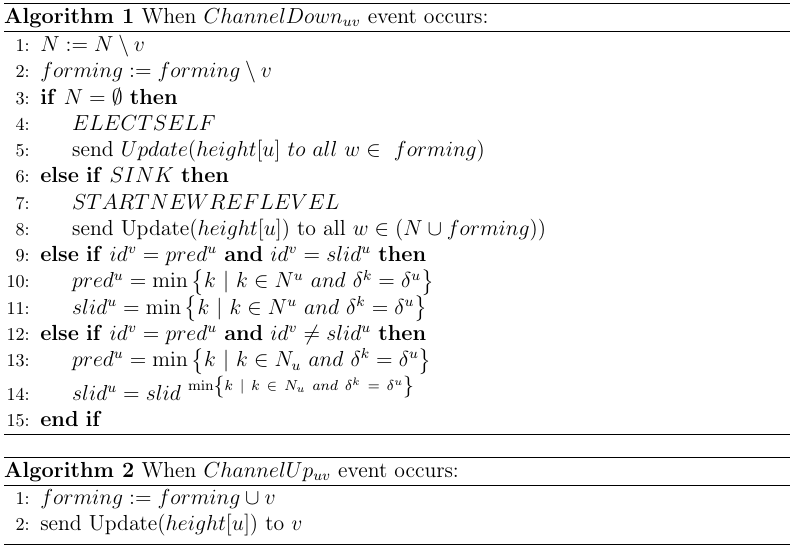
\includegraphics[width=0.8\linewidth]{channel_up_down.png}
	\caption{Code triggered by Topology Changes}
	\label{fig:figure1}
\end{figure}
\end{frame}

\begin{frame}
\begin{figure}[h]
	\centering
	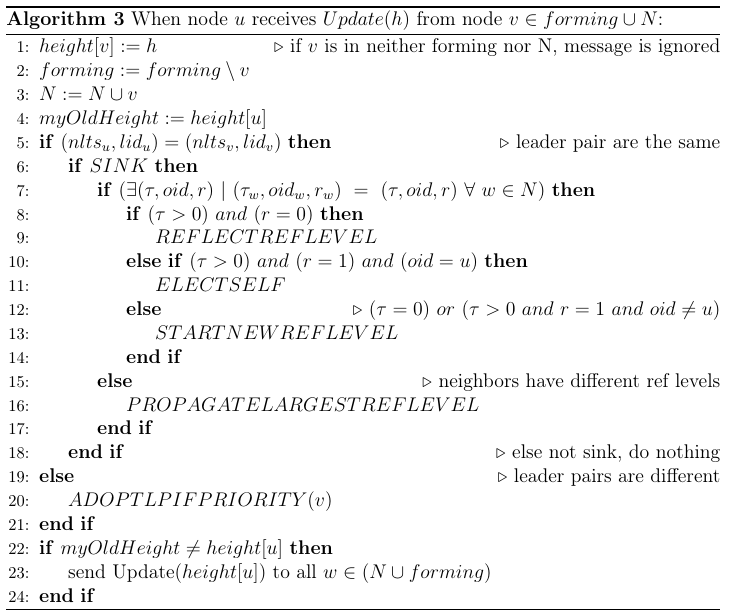
\includegraphics[width=0.7\linewidth]{message_received.png}
	\caption{Code triggered by Update Message}
	\label{fig:figure1}
\end{figure}
\end{frame}
\begin{frame}
\begin{figure}[h]
	\centering
	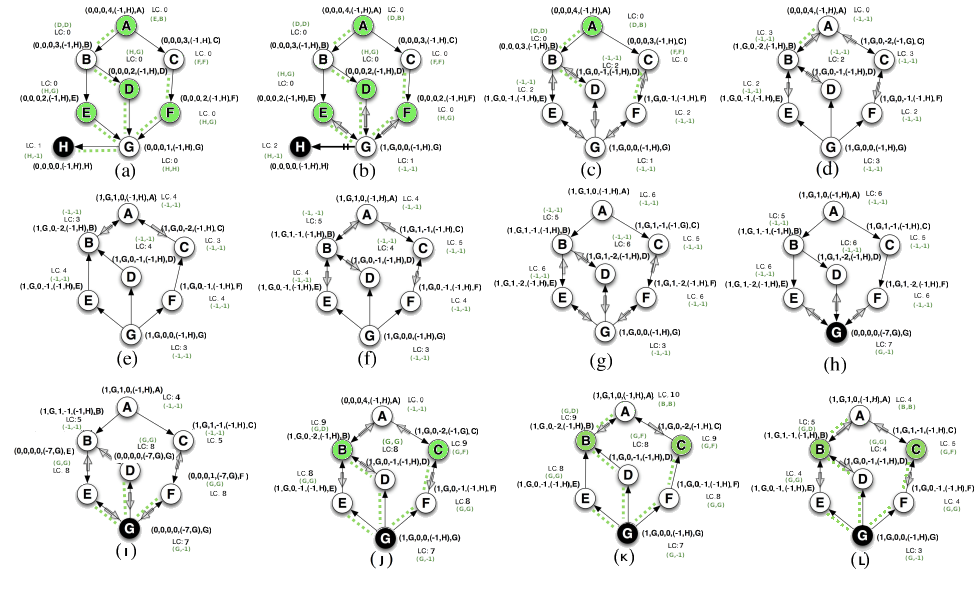
\includegraphics[width=0.9\linewidth]{sample_execution.png}
	\caption{Sample Execution}
	\label{fig:figure1}
\end{figure}
\end{frame}

\begin{frame}
\begin{figure}[h]
	\centering
	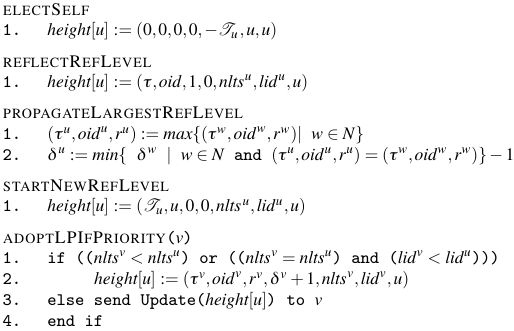
\includegraphics[width=0.75\linewidth]{subroutines.png}
	\caption{Subroutines}
	\label{fig:figure1}
\end{figure}
\end{frame}


% -----------------------------------------------------------------------------
\section{Correctness}
\begin{frame}{How the proof is dealt with ?}
	The proof uses a number of invariants, denoted as “Properties”, which are shown to hold in every configuration of every execution; each one is proved (separately) by induction on the configurations occurring in an execution.
\end{frame}


\subsection{Bounding the Number of Elections}

\begin{frame}{Bounding the Number of Elections}
	We bound, in Lemma 3, the number of elections that can occur after the last topology change; this result relies on the fact, shown in Lemma 2, that once a node u adopts a leader that was elected after the last topology change, u never becomes a sink again.
\end{frame}

\subsection{Bounding the Number of New Reference Levels}
\begin{frame}{Bounding the Number of Elections}
We bound, in Lemma 4, the number of new reference levels that are started after the last topology change; the proof of this result relies on several additional properties.
\end{frame}
\subsection{Bounding the Number of Messages}
\begin{frame}{Bounding the Number of Messages}
We show, in Lemmas 5, 6, and 7, that eventually there are no messages in transit and every node has an accurate view of its neighbors’ heights.
\end{frame}
\subsection{Proving The Leader-Oriented DAG Aspect}
\begin{frame}{Proving The Leader-Oriented DAG Aspect}
All the pieces are put together in Theorem 1 of Section 4.6 to show that eventually we have a leader-oriented connected component; a couple of additional properties are needed for this result.
\end{frame}
% -----------------------------------------------------------------------------

\section{Implementation}
\subsection{The Tool Used}

\begin{frame}{What's JBotSim ?}
JBoTSim is a java library that offers basic primitives for proto-typing, running, and visualizing distributed algorithms in dynamic networks.
\end{frame}

\subsection{Simulation}
\begin{frame}

  \animategraphics[loop,controls,width=\linewidth]{10}{output/out-}{0}{224}




\end{frame}

\subsection{Performance Test}

\begin{frame}{Performance Characteristics}
	\begin{enumerate}
		\item \textbf{Latency} $l$. The number of rounds necessary for a component to elect a leader (become stable) after a topology change (average over all initial topologies).
		
		\item \textbf{Sensitivity} $s$. The number of nodes that updated their heights in response to a topology change (average over all possible topology changes).
		
		\item \textbf{Resilience} $r$. The maximal fraction of links which can go down in a stable component without reelecting the current leader.
		
	\end{enumerate}
\end{frame}

\begin{frame}{Performance Characteristics}
\begin{itemize}
	\item Merging two stable components:
	\begin{itemize}
		\item Given two fully connected (every two nodes are neighbours) components: $l \simeq 2$.
		\item Given two poorly connected (a node can have not more than two neigh- bours) components: $l \simeq n$.
	\end{itemize}

	\item Partitioning a stable component:
	\begin{itemize}
		\item Getting two fully connected component: $l = 2$.
		\item Getting two poorly connected component: $l = 2n$.
	\end{itemize}
	

\end{itemize}
\end{frame}
\begin{frame}
	\begin{itemize}
		\item Topology change in a “small world-like” stable component (every node has O(log n) neighbours) without partitioning:
		\begin{itemize}
			\item Latency $l = O(1)$.
			\item Sensitivity $s = O(log(n))$.
		\end{itemize}
		\item Resilience of a stable component:
		\begin{itemize}
			\item Given a fully connected component: $r \simeq 1 - 2/n$.
			\item Given a “small world-like” component: $r \simeq 1 - 2/log(n)$.
		\end{itemize}
	\end{itemize}
\end{frame}


\begin{frame}{How is our algorithm's performance ?}
	\begin{figure}
		\centering
		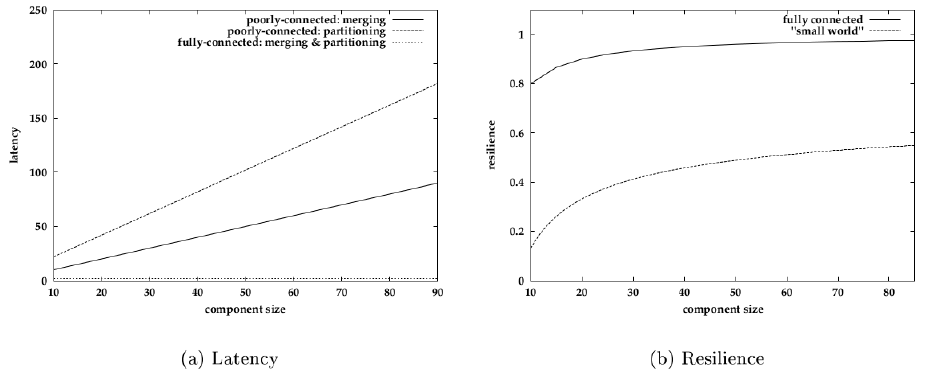
\includegraphics[width=1.1\linewidth]{performance_test}
		\caption{Simulation Results}
		\label{fig:performancetest}
	\end{figure}
	
\end{frame}

%----------------------------------------------------------------------------
\section{Conclusion}
\subsection{Is The Algorithm Perfect ?}
\begin{frame}{Is The Algorithm Perfect ?}
 \begin{itemize}
	\item  An open question is how to extend our algorithm and its analysis to handle a wider range of clocks, such as approximately synchronized clocks and vector clocks.
	\item Another question could be asked concerning the possibility of building up an optimized spanning tree using some algorithms such as Kruskal’s Minimum Spanning Tree Algorithm (MST).
 \end{itemize}

\end{frame}

\begin{frame}{Thank you for your attention}
	All your questions and remarks are welcomed.
\end{frame}
% -----------------------------------------------------------------------------
\end{document}
